\title{Associative Memory in Transformers:\\
Topology, Iterative Retrieval, and Controlled Activation with Progressive Retrieval Attention}
\author{Jorge Simao\\EInnovator R\&D -- Center for the Sciences of Computation, Cognition, and Complexity}
\date{\today}
\hypersetup{pdftitle={Associative Memory in Transformers},pdfauthor={Jorge Simao}}

\begin{document}
\maketitle

\begin{abstract}
Global self-attention can contextualize distant evidence while making the resulting memory geometry
less explicitly traversable.  We use Progressive Retrieval Attention (PRA) to ask whether transformer
states expose an associative topology, whether iterative retrieval can traverse it, and where useful
retrieval fails to influence computation.  A controlled family of 25 matched causal decoders varies
only the training attention window $W\in\{16,32,64,128,\mathrm{global}\}$ across five seeds.  Each
checkpoint is converted without learning to native-K/V PRA.  We complement this causal study with
frozen Qwen, Gemma, and Llama-family diagnostics on multi-hop language tasks.

At the controlled model's final layer, $W=16$ attains native edge R@4 $.428\pm.076$, versus
$.187\pm.065$ under global attention.  Under the same 20 layer-token K/V budget, evolving-state
iterative PRA improves complete-path recovery over one-shot retrieval in 59/400 (14.8\%)
model--example units.  Within this path-improved subset, correct-label margin increases by $2.164$,
with a paired-bootstrap 95\% interval $[1.336,2.971]$, while aggregate answer-accuracy improvement
remains statistically unresolved.  Ordinary executable memory is distractor dominated, assigning
.147 final-query
attention mass to evidence and .521 to memory distractors.  A matched oracle intervention raises
frozen accuracy from .140 to .398 and correct-label margin from $-3.103$ to $-.703$.

These results identify controlled activation, not absolute frozen-consumer incapacity, as the
dominant limitation.  Transformer memory contains topology that depends causally on receptive field;
iterative PRA can traverse that topology; and the frozen computation can use correctly activated
memory.  The unresolved problem is to make useful evidence dominate sparse external-memory influence
and to preserve that influence through subsequent layers.
\end{abstract}

\section{Introduction}

If attention provides associative access to contextual memory, does a transformer preserve a
traversable memory topology, and can sparse iterative activation exploit it?  Consider a query that
directly identifies memory $A$, while $A$ supplies the relation needed to find memory $B$.  One-shot
retrieval may rank $A$ but miss $B$ because the initial query does not yet contain the intermediate
relation.  Raising top-$k$ can recover $B$ accidentally, at the cost of activating more unrelated
memory.  Iterative retrieval instead asks whether $A$ itself can become a new search state.

This question has two parts that are often conflated.  First, the model must expose useful
memory-to-memory geometry.  Second, selected memories must influence the residual stream in the
right direction.  A recovered path can fail at either boundary: routing can select distractors, the
shared softmax can assign them most of the memory mass, or later layers can erase an initially useful
change.  Conversely, a weak aggregate output effect does not prove that associative traversal or
frozen memory consumption is absent.

PRA separates compact routing state from layer-native K/V payloads
\cite{simao2026pra,simao2026position,simao2026hf}.  That separation lets us observe root activation,
associative traversal, physical activation, attention allocation, residual change, and final output
as distinct events.  It also enables a strict comparison: one-shot and evolving-state iterative PRA
receive the same layer-token K/V budget, and selected URI identities cannot be replayed merely to
consume another intervention.

The paper has four principal findings.  First, local receptive fields preserve stronger explicit
native Q/K topology than global attention.  Second, matched iterative PRA exploits that topology to
recover more complete paths.  Third, better traversal is functionally useful when it changes selected
evidence: correct-answer margin rises substantially in the path-improved subgroup.  Fourth, ordinary
activation remains noisy, whereas matched oracle memory produces a large frozen-model output gain.
Table~\ref{tab:headline-questions} states the resulting causal decomposition.

\begin{table}[H]
\centering
\caption{Headline questions, results, and consequences.  Controlled values use five receptive-field
settings and five seeds unless explicitly described as model--example diagnostics.}
\label{tab:headline-questions}
\scriptsize
\begin{tabular}{p{0.31\linewidth}p{0.27\linewidth}p{0.34\linewidth}}
\toprule
Scientific question & Result & Consequence \\
\midrule
Does transformer memory expose associative topology? & Yes: native Q/K contains recoverable evidence edges & Compact states support explicit traversal. \\
Does receptive field affect topology? & Yes: final-layer R@4 is .428 at $W=16$ and .187 globally & Locality preserves stronger explicit structure. \\
Can iterative PRA traverse it? & Yes: path recovery usually rises at the same 20-state budget & Evolving-state access is an operational primitive. \\
Does improved traversal help computation? & Yes when useful evidence changes: margin $+2.164$ & Traversal is useful, but improved cases are sparse. \\
Why is aggregate answer gain weak? & Selected memory gives .147 mass to evidence and .521 to distractors & Controlled activation is the dominant bottleneck. \\
Can the frozen model consume correct PRA memory? & Yes: oracle accuracy .140$\rightarrow$.398 & Frozen-consumer incapacity is rejected as an absolute explanation. \\
Do layers matter? & Yes: search, consumption, and preservation profiles differ & There is no universal best PRA layer. \\
\bottomrule
\end{tabular}
\end{table}

Our contributions are: (1) controlled causal evidence that receptive field shapes associative
topology; (2) matched-budget evidence that evolving-state PRA traverses that topology; (3) a causal
decomposition of retrieval, attention allocation, residual change, and preservation; (4) oracle
evidence that frozen transformers can use correctly activated external memory; and (5) pretrained
validation of root-entry, granularity, layer, and distractor-competition effects.  The chronological
mechanism search, including negative results, remains intact in the appendices.

\section{PRA as a Probe of Associative Memory}

Let $G=\{g_1,\ldots,g_N\}$ be compact routing gists at one transformer layer and let $q$ be the
current query state.  One-shot PRA returns
\begin{equation}
  N_B(q)=\operatorname{TopB}_{g\in G}s(q,g).
\end{equation}
This is sufficient when each useful memory is independently similar to $q$.  It is incomplete when
\begin{equation}
  s(q,g_A)\gg0,\qquad s(q,g_B)\approx0,\qquad s(g_A,g_B)\gg0.
\end{equation}
Here $A$ is the \emph{root activation}: the first query-to-memory transition.  The transition
$A\rightarrow B$ is \emph{associative traversal}.  PRA performs this search over compact state and
activates full layer-native K/V only for the final selected identities.

Five terms remain distinct throughout the paper.  \emph{Associative topology} is the native Q/K
geometry linking memory states.  \emph{Controlled activation} selects a working set in which useful
evidence can dominate external-memory influence.  \emph{Consumption} converts attended memory into
a useful residual or output change.  \emph{Preservation} or \emph{assimilation} asks whether that
change survives later transformer computation.  Selection is therefore not equivalent to attention,
and attention is not equivalent to useful output.

At a PRA layer, memory and direct-context K/V share one softmax.  For the final query token we measure
\begin{equation}
  A_E=\sum_{j\in\mathrm{evidence}}\alpha_j,\quad
  A_J=\sum_{j\in\mathrm{memory\ distractors}}\alpha_j,\quad
  A_N=\sum_{j\in\mathrm{native\ context}}\alpha_j,quad
  A_E+A_J+A_N=1.
\end{equation}
This decomposition exposes whether a correct identity merely appears in the working set or actually
competes successfully for influence.

\begin{figure}[H]
\centering
\fbox{\begin{minipage}{0.92\linewidth}
\centering
logical source or long prompt\\
$\downarrow$ model-safe encoding blocks $\downarrow$\\
layer-native K/V \quad+\quad contextual chunks and compact gists\\
$\downarrow$ root activation: $q\rightarrow A$ $\downarrow$\\
associative traversal: $A\rightarrow B\rightarrow C$\\
$\downarrow$ bounded identity selection $\downarrow$\\
selected native K/V $\rightarrow$ shared-softmax direct + memory attention\\
$\downarrow$ residual assimilation $\downarrow$\\
frozen transformer output
\end{minipage}}
\caption{PRA as an associative-memory probe.  Compact search and full native-K/V activation are
separate phases, so topology, traversal, activation, consumption, and preservation can be measured
independently.}
\label{fig:pra-probe}
\end{figure}

\section{Controlled Model: Receptive Field and Memory Topology}
\label{sec:controlled-local}

\subsection{Controlled task and model family}

Each example samples a fresh entity/relation chain of depth $D\in\{1,2,3,4\}$.  The terminal entity
maps to one of eight balanced labels, so chance accuracy is .125.  Facts contain five tokens and the
query contains a start entity plus a relation sequence; the standalone PRA query has $D+4$ tokens
including \texttt{[BOS]} and never includes the answer.  In the mechanistic cohort, distractor
interleaving and controlled gaps produce 7--55-token evidence spans and 5--11-token maximum hop
distances.  The artifacts record these quantities and their ratios to $W$ for every paired example.

Multiple distractors use the same terminal relation with wrong source entities, preventing a unique
relation scan from solving the task.  Evidence appears only in reverse causal order, while distractors
are randomly interleaved.  Train, validation, test, topology, and PRA corpora use disjoint deterministic
seeds and are shared across every model seed and $W$.  Gold paths are joined only after inference and
never enter cache metadata or executable selection.

\begin{figure}[H]
\centering
\fbox{\begin{minipage}{0.90\linewidth}
\centering
query: start entity + relation sequence \qquad answer: one of 8 balanced labels\\[3pt]
$\downarrow$\\[-2pt]
randomly interleaved five-token facts: evidence chain + matched relation distractors\\[3pt]
$\downarrow$\\[-2pt]
matched 6-layer decoder with $W\in\{16,32,64,128,\mathrm{global}\}$\\[3pt]
$\downarrow$\\[-2pt]
native Q/K edge ranks, path survival, contextual dependence, and answer prediction
\end{minipage}}
\caption{Controlled scientific instrument.  Only the native training attention window varies across
the five model families; corpus, architecture, optimization, and evaluation remain matched.}
\label{fig:controlled-task}
\end{figure}

\begin{table}[H]
\centering
\caption{Controlled model and data configuration.}
\label{tab:controlled-config}
\small
\begin{tabular}{p{0.31\linewidth}p{0.58\linewidth}}
\toprule
Property & Fixed value \\
\midrule
Decoder & 6 pre-norm layers, width 96, 4 heads, FFN width 384, RoPE, no dropout \\
Parameters / vocabulary & 739,968 / 230 controlled tokens \\
Native attention & $W\in\{16,32,64,128,\mathrm{global}\}$; the current token is included \\
Train / validation / test & 4,096 / 512 / 512 disjoint deterministic examples \\
Optimization & AdamW, batch 48, 800 updates, gradient norm 1.0, warmup plus cosine decay \\
Checkpoint rule & Validation accuracy every 100 updates; loss breaks ties; test remains untouched \\
Initialization seeds & 17, 29, 41, 53, 67 \\
\bottomrule
\end{tabular}
\end{table}

A one-layer local mask exposes at most the current token and previous $W-1$ positions.  Across $L$
layers, theoretical causal reach can grow to $1+L(W-1)$ tokens.  We therefore do not equate a local
mask with permanently isolated state.  Native edge metrics and restricted-context interventions are
measured at every layer and compared with actual evidence span and hop distance.

\subsection{Native topology depends on receptive field}

For every evidence edge $A\rightarrow B$, we score $A$'s native per-head query against mean native
keys for all facts.  Table~\ref{tab:controlled-native-results} reports held-out model behavior and
final-layer topology.  The output threshold lies near $W=32$, while explicit topology moves in the
opposite direction: R@4 declines from .428 at $W=16$ to .187 globally and shortcut rate rises from
.429 to .584.  Complete four-hop survival at R@4 is .203 at $W=16$ and .119 globally.

\begin{table}[H]
\centering
\caption{Held-out quality and final-layer native topology.  Intervals are five-seed Student-$t$
95\% intervals.}
\label{tab:controlled-native-results}
\small
\begin{tabular}{lrrrr}
\toprule
Window & Test accuracy & Test loss & Edge R@4 & Shortcut rate \\
\midrule
$16$ & $.415\pm.030$ & 1.767 & $.428\pm.076$ & $.429\pm.027$ \\
$32$ & $.511\pm.012$ & 1.218 & $.294\pm.072$ & $.524\pm.052$ \\
$64$ & $.506\pm.020$ & 1.118 & $.277\pm.039$ & $.497\pm.061$ \\
$128$ & $.514\pm.010$ & 1.077 & $.196\pm.062$ & $.537\pm.080$ \\
Global & $.522\pm.017$ & 1.085 & $.187\pm.065$ & $.584\pm.069$ \\
\bottomrule
\end{tabular}
\end{table}

\begin{figure}[H]
\centering
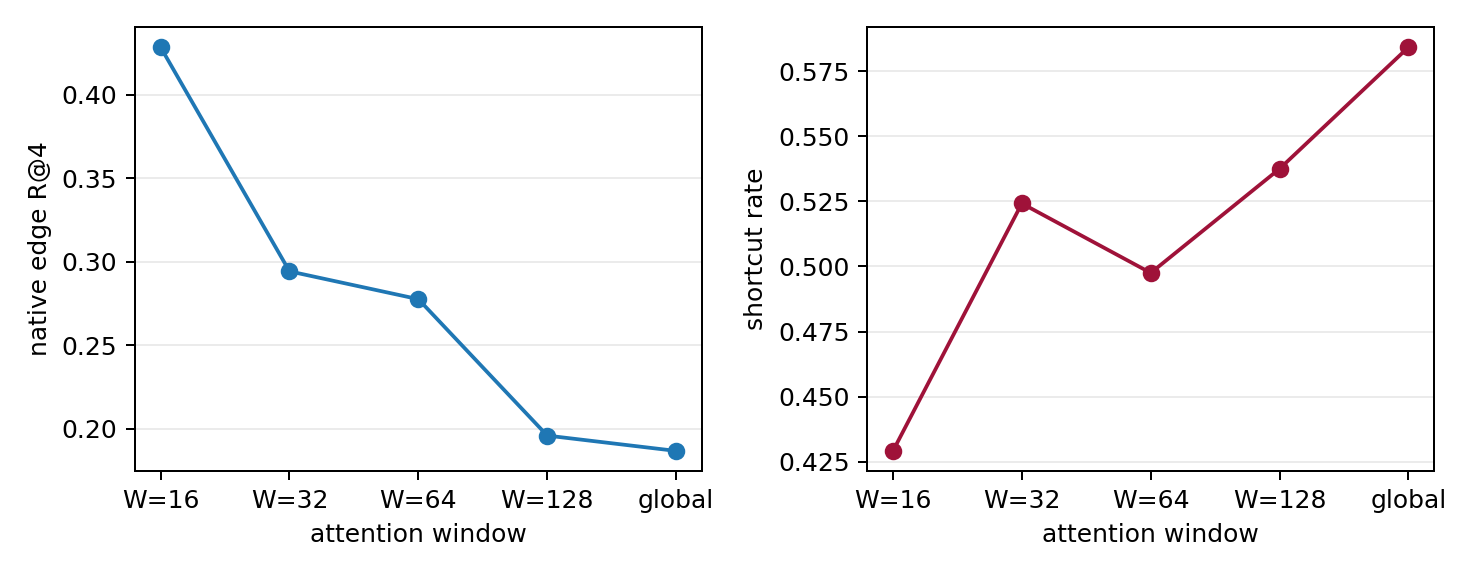
\includegraphics[width=0.88\linewidth]{../shared/results/paper2_5_iterative_pra/controlled_local_sa_v6/figures/outcome_b/topology_vs_window.png}
\caption{Native edge R@4 and shortcut rate across the matched receptive-field family.  The trend is
smooth rather than a $W=16$ endpoint artifact.}
\label{fig:controlled-native-window}
\end{figure}

\subsection{Contextualization is not traversability}

For $W=16$, R@4 rises from .221 at layer 0 to .408 at layer 1 and remains near .4, while dependence
on context outside the final 16 tokens grows from approximately zero to .426.  Global restricted-
context dependence approaches .494 while R@4 remains near .2.  Local states therefore accumulate
context through depth without converging to the global model's shortcut-rich topology.

\begin{figure}[H]
\centering
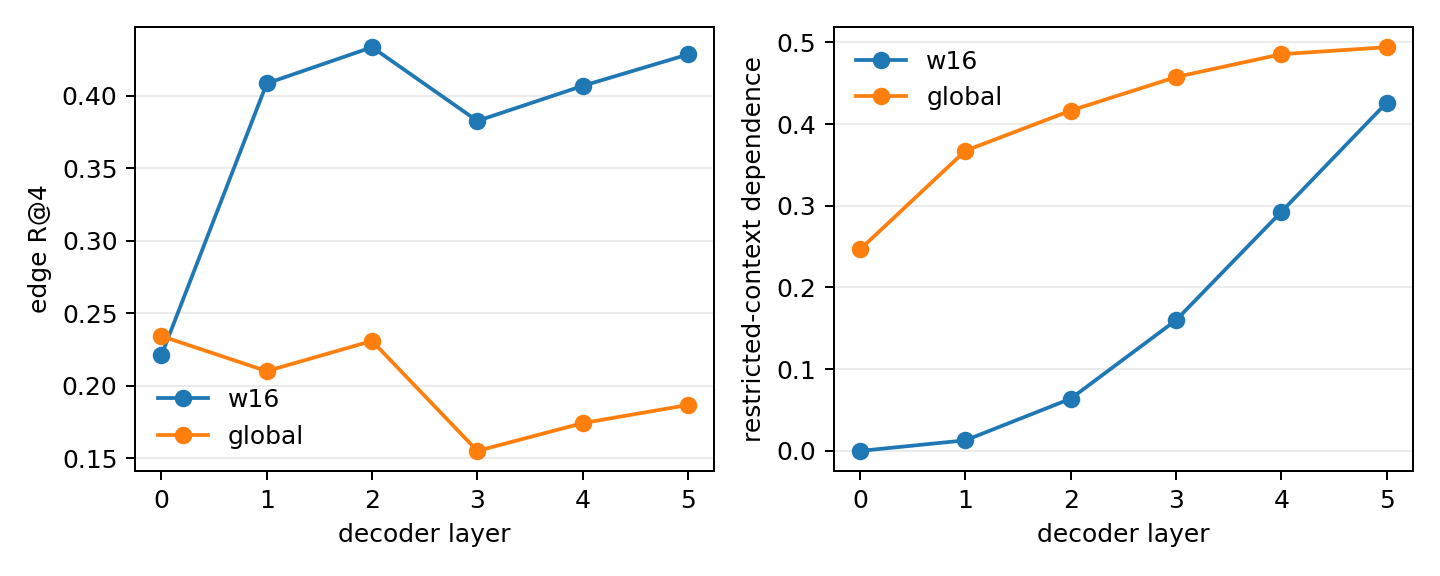
\includegraphics[width=0.84\linewidth]{../shared/results/paper2_5_iterative_pra/controlled_local_sa_v6/figures/layerwise_topology_context.png}
\caption{Layerwise edge R@4 and restricted-context dependence.  More contextualized does not mean
more explicitly traversable.}
\label{fig:controlled-layerwise}
\end{figure}

\section{Controlled Iterative Retrieval}

\subsection{Evolving-state retrieval under a matched physical budget}

After training, selected self-attention blocks are replaced with PRA blocks carrying the same layer
normalization, Q/K/V/O projections, and FFN weights.  Disabled-memory logits match the source model
to numerical tolerance.  One-shot PRA selects four facts at one layer.  Matched iterative PRA
selects one unseen fact at layers 0, 2, 4, and 5.  Both materialize exactly 20 layer-token K/V states.
The later query is the transformed hidden state after previous memory integration and intervening
self-attention/FFN computation:
\begin{equation}
 h_{\ell_1}\xrightarrow{\mathrm{PRA}(A)}h'_{\ell_1}
 \xrightarrow{\mathrm{SA/FFN}}h_{\ell_2}
 \xrightarrow{\mathrm{PRA}(B)}h'_{\ell_2}.
\end{equation}
Visited URI identities are removed from later caches, so iterative depth cannot be simulated by
replaying the first selected fact.

\begin{table}[H]
\centering
\caption{Matched one-shot and iterative PRA over in-domain depths 1--4.  Acc. is answer accuracy,
Rec. is evidence recall, and Path is complete-path recovery.}
\label{tab:controlled-pra-results}
\small
\begin{tabular}{lrrrrrrr}
\toprule
& \multicolumn{3}{c}{One-shot, 20 states} & \multicolumn{3}{c}{Iterative, 20 states} & $\Delta$ Acc. \\
Window & Acc. & Rec. & Path & Acc. & Rec. & Path & Iter.-one \\
\midrule
$16$ & .167 & .349 & .109 & .164 & .388 & .177 & -.004 \\
$32$ & .183 & .365 & .113 & .256 & .383 & .166 & +.073 \\
$64$ & .178 & .378 & .177 & .195 & .412 & .165 & +.018 \\
$128$ & .212 & .405 & .190 & .234 & .451 & .232 & +.021 \\
Global & .212 & .420 & .197 & .177 & .453 & .221 & -.036 \\
\bottomrule
\end{tabular}
\end{table}

Iterative retrieval raises path recovery in four of five windows, including +.068 at $W=16$, but
every five-seed accuracy interval crosses zero.  The largest mean answer difference is +.073 at
$W=32$, with a 95\% interval of $\pm.151$.  This does not mean graph traversal is irrelevant.  It
means the executable policy changes useful evidence too infrequently to establish a stable
architecture-level answer gain.

\begin{figure}[H]
\centering
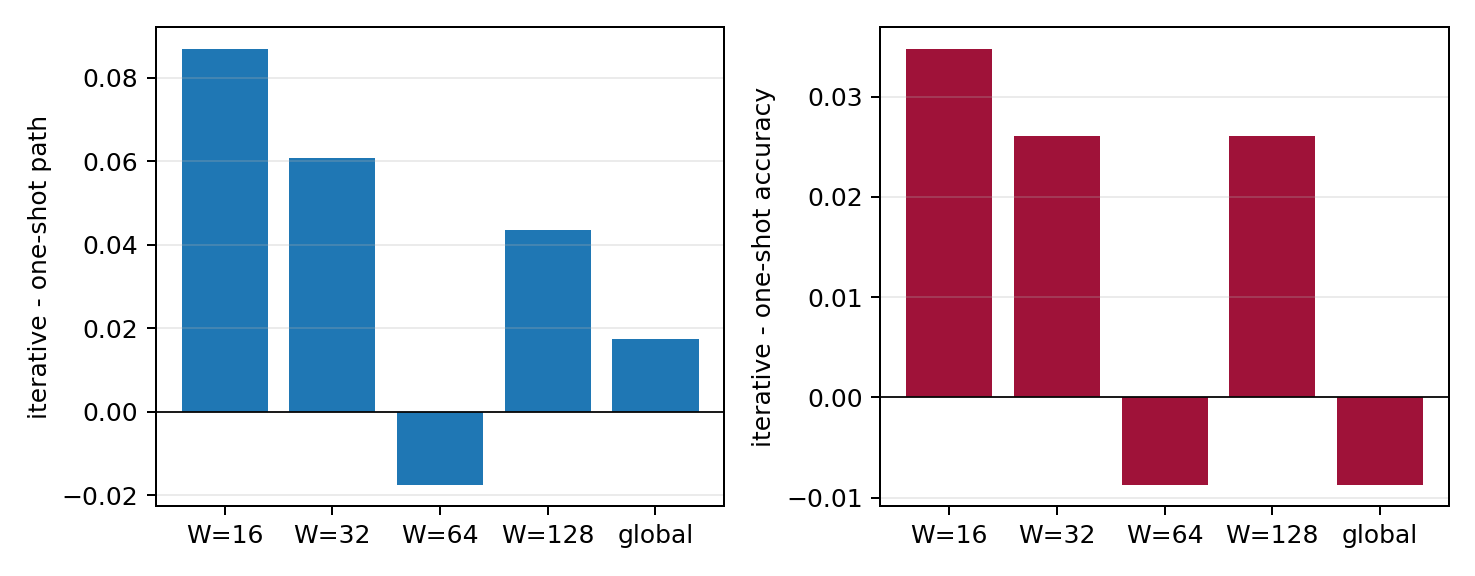
\includegraphics[width=0.86\linewidth]{../shared/results/paper2_5_iterative_pra/controlled_local_sa_v6/figures/outcome_b/traversal_answer_boundary.png}
\caption{Matched iterative-minus-one-shot path and answer changes by receptive field.  Traversal
improves more consistently than aggregate answer accuracy.}
\label{fig:traversal-answer-boundary}
\end{figure}

\subsection{Intervention density is a diagnostic frontier}

PRA at every layer averages 29.8 layer-token states and raises recovery further, but it is no longer
budget matched.  Sparser spacing reduces cost to 15, 10, and 5 states and generally reduces path
recovery.  Answer accuracy is non-monotonic.  More interventions make memory more active and alter
the residual stream; they do not guarantee more useful computation.

\begin{figure}[H]
\centering
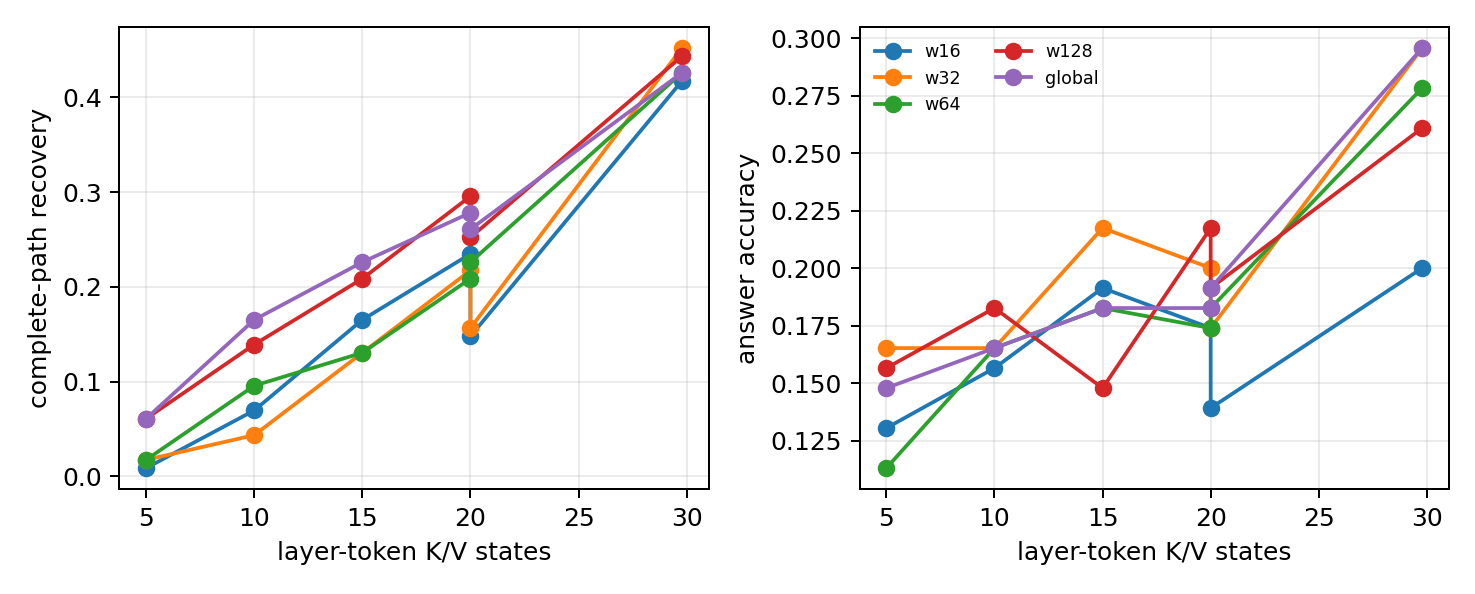
\includegraphics[width=0.86\linewidth]{../shared/results/paper2_5_iterative_pra/controlled_local_sa_v6/figures/outcome_b/intervention_density_frontier.png}
\caption{Layer-token K/V states versus complete-path recovery and answer accuracy.  Every-layer PRA
is retained as a diagnostic frontier, not a deployment policy.}
\label{fig:intervention-frontier}
\end{figure}

\section{Controlled Activation: Why Better Retrieval Sometimes Fails}
\label{sec:controlled-activation}

The matched traversal result identifies a boundary but not its cause.  We therefore reuse all 25
validation-selected checkpoints as frozen experimental instruments.  The causal cohort contains 16
paired held-out examples per checkpoint, or 400 model--example units.  No backbone, router, readout,
or memory projection is updated.

For the same model, query, layers, example, and physical budget, we compare no memory $E_0$;
ordinary selected memory $E_+$; oracle evidence plus enough unique distractors to preserve 20 states
$E_{\mathrm{oracle}}$; four non-evidence facts $E_{\mathrm{wrong}}$; and selected URI/gist identities
whose native K/V payloads are rotated among facts $E_{\mathrm{shuffle}}$.  Oracle identities are
available only to the named intervention and never to executable retrieval.

\subsection{Ordinary selected memory is distractor dominated}

Table~\ref{tab:causal-memory} is the central causal result.  Ordinary iterative selection raises
accuracy only from .140 to .195.  It assigns .147 attention mass to evidence and .521 to memory
distractors.  Shuffling leaves accuracy at .193, indicating that some selected-memory benefit is a
generic state perturbation or correlated selection effect rather than content-specific evidence use.

\begin{table}[H]
\centering
\caption{Frozen-consumer controls averaged equally over windows.  Every nonzero row uses exactly 20
layer-token K/V states.}
\label{tab:causal-memory}
\small
\begin{tabular}{lrrrrr}
\toprule
Memory condition & Complete path & Accuracy & Margin & Evidence mass & Distractor mass \\
\midrule
$E_0$ & .000 & .140 & $-3.103$ & .000 & .000 \\
$E_+$ & .408 & .195 & $-2.255$ & .147 & .521 \\
$E_{\mathrm{oracle}}$ & 1.000 & .398 & $-.703$ & .270 & .301 \\
$E_{\mathrm{wrong}}$ & .000 & .058 & $-3.544$ & .000 & .546 \\
$E_{\mathrm{shuffle}}$ & .418 & .193 & $-2.318$ & .122 & .433 \\
\bottomrule
\end{tabular}
\end{table}

\begin{figure}[H]
\centering
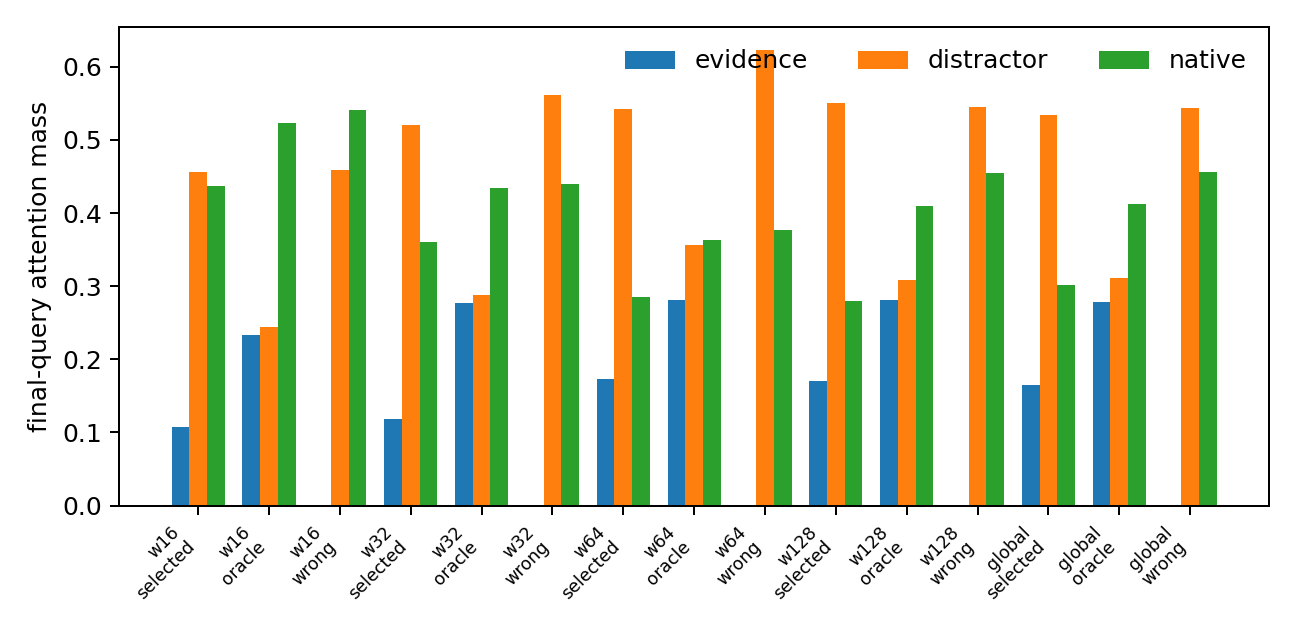
\includegraphics[width=0.88\linewidth]{../shared/results/paper2_5_iterative_pra/controlled_local_sa_v6/figures/outcome_b/memory_attention_decomposition.png}
\caption{Exact final-query shared-softmax decomposition.  Executable selected memory is consistently
distractor dominated; matched oracle forcing increases evidence mass while preserving budget.}
\label{fig:memory-mass}
\end{figure}

\subsection{Oracle memory establishes consumption capacity}

Oracle forcing raises complete-path recovery to 1.0, accuracy to .398, and margin from $-3.103$ to
$-.703$.  Accuracy improves in 23 of 25 window--seed pairs and margin in 24 of 25.  With five seeds
per window, the strongest exact two-sided sign result is still $p=.0625$; the result is a large,
directionally consistent causal ceiling, not a fully powered deployment comparison.  Wrong memory
lowers accuracy to .058.  Memory content therefore matters, and the frozen transformer has
substantial latent capacity to consume correctly activated PRA memory.

\begin{figure}[H]
\centering
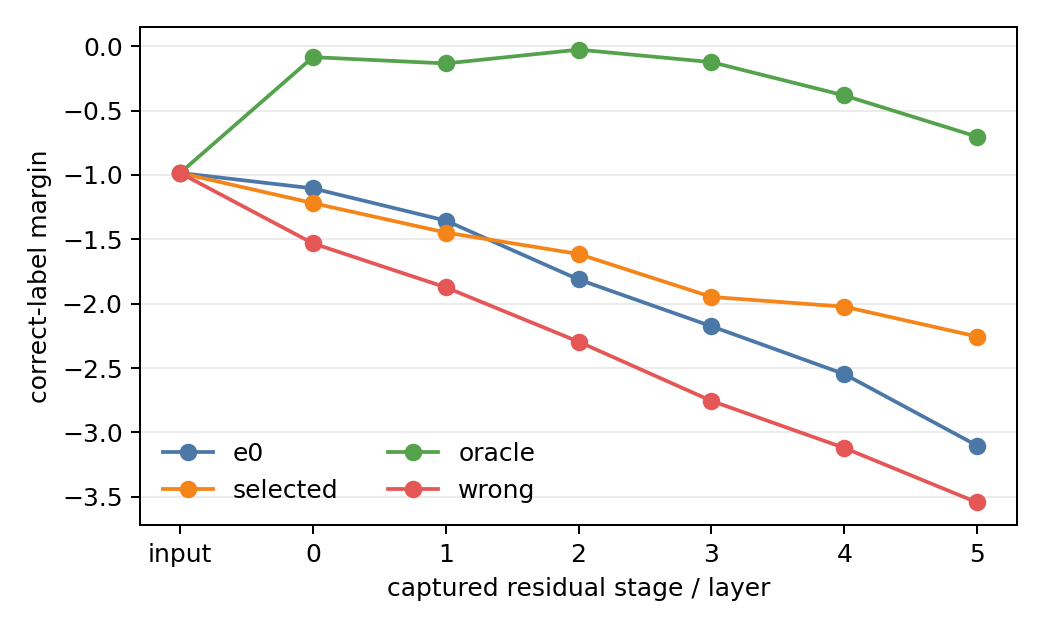
\includegraphics[width=0.72\linewidth]{../shared/results/paper2_5_iterative_pra/controlled_local_sa_v6/figures/outcome_b/answer_margin_trajectory.png}
\caption{Correct-label margin through the frozen residual stack for no memory, ordinary selected,
oracle, and wrong memory.  Oracle evidence separates early; wrong memory moves in the opposite
direction.  Curves average paired checkpoints and examples for diagnosis rather than calibration.}
\label{fig:margin-trajectory}
\end{figure}

\subsection{When does iteration help?}

Iterative PRA improves complete-path recovery over one-shot in 59 of 400 model--example units,
leaves it unchanged in 293, and worsens it in 48.  Within the improved subset, correct-label margin
rises by 2.164 with paired bootstrap 95\% interval $[1.336,2.971]$; accuracy rises by .102 with
interval $[-.017,.220]$.  When path recovery worsens, margin falls by 1.585 and accuracy by .292.
Across all rows, path gain correlates .279 with margin gain and .207 with answer gain.  Better
traversal is therefore functionally useful when it changes evidence, but the tested policy does not
produce that event reliably enough for a stable aggregate accuracy improvement.

Let $G_+=\{\Delta\mathrm{path}>0\}$ denote the 59 improved units and
$G_0=\{\Delta\mathrm{path}\leq0\}$ the other 341.  Table~\ref{tab:iteration-benefit}
compares their existing traces.  The first block contains measurements available after one-shot
retrieval but before choosing a retry; the second contains consequences observed only after
iteration.  The distinction matters: margin gain, iterative evidence mass, and erasure can diagnose
a completed retry but cannot serve as deployable retry triggers.

\begin{table}[H]
\centering
\caption{Path-improved versus other model--example units.  Entries are means; $d$ is the pooled
standardized mean difference except for answer gain, reported as a mean change.  Intervals
and medians are preserved in the public derived CSV.}
\label{tab:iteration-benefit}
\small
\begin{tabular}{llrrr}
\toprule
Timing & Feature & $G_+$ (59) & $G_0$ (341) & Effect \\
\midrule
Pre-decision & One-shot reference recall & .085 & .603 & $d=-1.393$ \\
Pre-decision & One-shot evidence mass & .037 & .230 & $d=-1.094$ \\
Pre-decision & One-shot distractor mass & .871 & .657 & $d=1.119$ \\
Pre-decision & Chain depth & 1.17 & 1.92 & $d=-.770$ \\
Pre-decision & One-shot margin & $-4.137$ & $-2.330$ & $d=-.534$ \\
Pre-decision & Evidence span (tokens) & 30.83 & 26.92 & $d=.307$ \\
\midrule
Post-treatment & Margin gain & 2.164 & .026 & $d=.629$ \\
Post-treatment & Answer gain & .102 & $-.065$ & $+.166$ \\
Post-treatment & Iterative evidence mass & .202 & .137 & $d=.635$ \\
Post-treatment & Iterative distractor mass & .476 & .528 & $d=-.387$ \\
Post-treatment & Erased by final layer & .203 & .185 & $p=.720$ \\
\bottomrule
\end{tabular}
\end{table}

One-shot complete-path recovery is zero in every $G_+$ unit by construction: a binary complete path
cannot improve from one.  That fact identifies retry eligibility, not a learned signature.  Among
the 248 one-shot misses, 59 improve and 189 do not.  Relative to those 189 misses, improved retries
have shorter chains (1.17 versus 2.50, $d=-1.43$), longer evidence spans (30.83 versus 20.94 tokens,
$d=.89$), less one-shot evidence mass (.037 versus .156, $d=-.779$), and more distractor mass (.871
versus .720, $d=.854$).  Their baseline margin is also lower ($-4.137$ versus $-3.233$, $d=-.319$).
Thus the minority has a recognizable controlled-task profile: shallow recoverable paths whose
one-shot working set is especially evidence poor.  Query length is omitted from the interpretation
because this synthetic generator couples it to chain depth.  Root-score gaps, routing entropy,
facets, per-unit native R@$K$/MRR, contraction, and frontier competition were not recorded for these
paired units.

We do not fit a retry classifier.  The cohort contains only 16 repeated task identities per
checkpoint, and its strongest features are either structural eligibility or generator-coupled.
Treating a random row split across seeds as independent prediction would overstate generalization.
The descriptive signature instead motivates the independent adaptive-control question in Paper 3.5.

\begin{figure}[H]
\centering
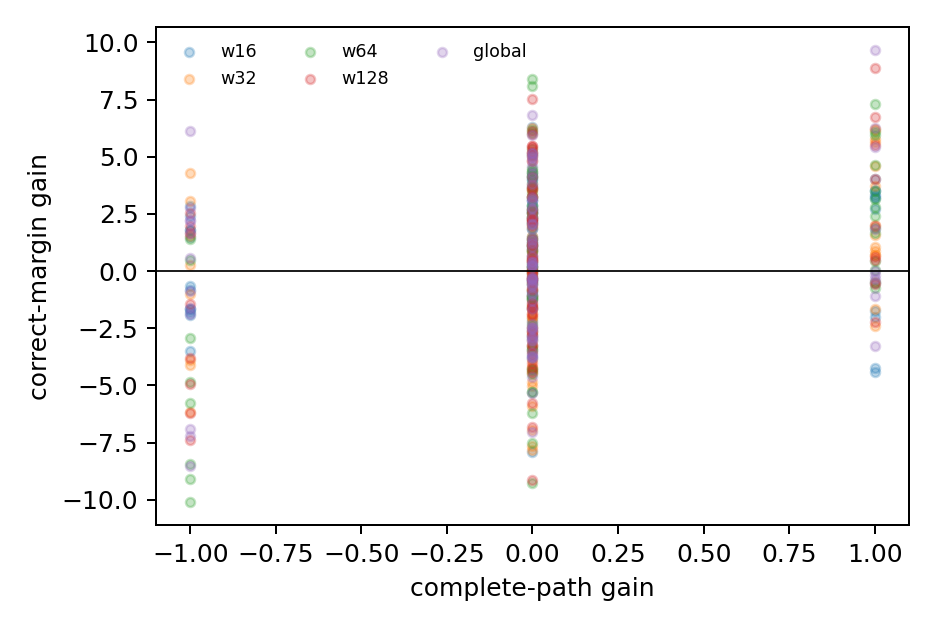
\includegraphics[width=0.62\linewidth]{../shared/results/paper2_5_iterative_pra/controlled_local_sa_v6/figures/outcome_b/path_gain_margin_gain.png}
\caption{Paired complete-path and correct-margin changes.  Positive path changes usually move the
frozen decision in the correct direction, but most rows do not improve the path.}
\label{fig:path-margin-gain}
\end{figure}

\begin{table}[H]
\centering
\caption{Causal diagnosis from associative topology to preserved output.}
\label{tab:causal-diagnosis}
\scriptsize
\begin{tabular}{p{0.20\linewidth}p{0.34\linewidth}p{0.36\linewidth}}
\toprule
Stage & Finding & Interpretation \\
\midrule
Topology & Local $W$ preserves stronger R@K & Associative structure exists and depends on receptive field. \\
Traversal & Iterative PRA improves path recovery & The structure is operationally traversable. \\
Ordinary activation & Evidence mass .147, distractor mass .521 & Executable selection is noisy. \\
Oracle activation & Accuracy .140$\rightarrow$.398; margin $-3.103\rightarrow-.703$ & Frozen computation can use correct memory. \\
Improved-path subset & Margin $+2.164$ & Better traversal is useful when selected evidence changes. \\
Later computation & 21.6\% of initially positive oracle traces are erased & Scheduling and assimilation are secondary limits. \\
\bottomrule
\end{tabular}
\end{table}

\section{Layer Dynamics: Search, Consumption, and Preservation}

The best search layer $L_{\mathrm{search}}$ is where native Q/K ranks useful successors well.  The
best consumer layer $L_{\mathrm{consume}}$ is where fixed oracle memory most improves the answer
state.  A preservation profile asks whether the resulting gain survives later layers.  These are
different measurements and need not peak together.

Oracle usefulness is strongest early in this controlled family.  Averaged across windows, injection
at layer 0 gives .358 accuracy and $-1.239$ margin, compared with .138 and $-2.565$ at layer 5.  The
native graph-search optimum follows a different layer ordering.  Among oracle traces with a positive
immediate margin effect, 21.6\% lose that advantage by the final layer.  Mean local answer-direction
alignment is positive for oracle memory (.054), near zero for selected memory (.017), and negative
for wrong memory ($-.061$).  Evidence value-contribution norm rises from 1.283 under ordinary
selection to 2.105 under oracle selection.

\begin{figure}[H]
\centering
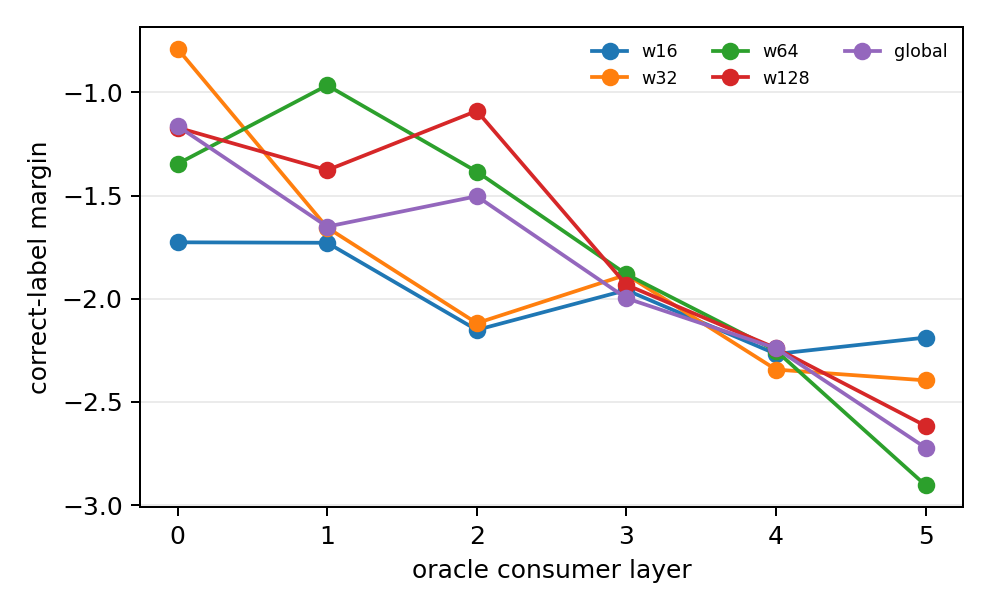
\includegraphics[width=0.78\linewidth]{../shared/results/paper2_5_iterative_pra/controlled_local_sa_v6/figures/outcome_b/oracle_consumer_layer.png}
\caption{Oracle consumer-layer profile.  Early layers use the same correct memory more effectively
than late layers, while native graph quality has a separate, non-monotonic profile.}
\label{fig:consumer-layer}
\end{figure}

\begin{figure}[H]
\centering
\fbox{\begin{minipage}{0.88\linewidth}
\centering
\textbf{QUERY / CURRENT STATE}\\
$\downarrow$\\
\textbf{ROOT ACTIVATION}\\
$\downarrow$\\
\textbf{ASSOCIATIVE TRAVERSAL} \quad ($W=16$ path $+.068$ at matched budget)\\
$\downarrow$\\
\textbf{SELECTED MEMORY}\\
$\searrow$ distractors dominate (.521 vs .147 evidence) $\rightarrow$ poor activation\\
$\downarrow$\\
\textbf{EVIDENCE-DOMINATED ATTENTION} \quad (oracle evidence mass .270)\\
$\downarrow$\\
\textbf{USEFUL RESIDUAL CHANGE} \quad (path-improved margin $+2.164$)\\
$\searrow$ later erasure (21.6\%) $\rightarrow$ lost gain\\
$\downarrow$\\
\textbf{OUTPUT} \quad (oracle accuracy .140$\rightarrow$.398)
\end{minipage}}
\caption{Final causal pipeline.  The dominant measured loss is controlled activation between
selected memory and evidence-dominated attention; consumer placement and preservation are secondary.}
\label{fig:causal-pipeline}
\end{figure}

\section{Pretrained Validation}

The pretrained studies test whether the controlled decomposition remains useful in natural language.
They do not repeat the controlled causal intervention.  Qwen3-0.6B supplies the main frozen feature
and output artifacts; Gemma~3~1B and SmolLM2-135M provide architectural contrasts.  The latter is a
compact Llama-family model, not a Llama~3.x checkpoint.  Backbones, router checkpoints, post-RoPE
native K/V, and attention semantics remain fixed within each comparison.

Synthetic chains test exact transitive reachability.  QASPER is primarily a direct-evidence/root-entry
control; HotpotQA supplies bridge questions; 2Wiki supplies annotated evidence transitions; and
MuSiQue supplies deeper task graphs that reveal contraction.  These datasets have different roles and
are not pooled into one leaderboard.

\subsection{Root activation and query facets}

The all-offset audit shows that useful root-query views often exist but are hard to select.  Some
contextual span ranks a correct root in Top-4 for .878 MuSiQue and .950 2Wiki runs.  Fixed executable
facets achieve .422/.608; the best inexpensive held-out selectors reach .622/.692.  Position, hidden
norm, margin, entropy, and validation-fitted scale selectors do not close the gap.  Root activation is
therefore a competition problem, not simply the absence of a useful query representation.

HotpotQA makes that competition concrete.  A short bridge question can mix a source entity, first
relation, bridge object, second relation, and target property.  The correct first passage can be
necessary without being answer-like, so $\operatorname{sim}(Q,B)$ can exceed
$\operatorname{sim}(Q,A)$ even when $A$ is the correct root and $A\rightarrow B$ is a strong native
transition.  Distractors can match one sub-intent, and the query-to-memory comparison is asymmetric:
$Q$ is a question state while $A$ and $B$ are contextual memory states.  The inherited seven-identity
Hotpot test is not a failure case for candidate availability---global semantic root R@4 is .971---but
at a 20\% selection budget the correct root is included only .343 of the time.  Four-token contextual
facets raise inclusion to .457 by preserving relational subphrases, while comparisons rise from 5.9
to 67.6.  More facets create opportunities and competitors; selecting the facet that expresses the
current retrieval intention remains the hard part.

\begin{table}[H]
\centering
\caption{Held-out root Top-4 recall: oracle query view versus executable selection.}
\label{tab:main-entry}
\small
\begin{tabular}{lrr}
\toprule
Entry rule & MuSiQue & 2Wiki \\
\midrule
Deployed fixed facets & .422 & .608 \\
Bounded all-facet union & .411 & .475 \\
Best cheap selector & .622 & .692 \\
All-offset oracle ceiling & .878 & .950 \\
\bottomrule
\end{tabular}
\end{table}

\begin{table}[H]
\centering
\caption{Dataset routing geometry from frozen artifacts.  Values are diagnostic and cohorts differ
in role; blank oracle entries were not measured.}
\label{tab:dataset-routing-geometry}
\scriptsize
\setlength{\tabcolsep}{3pt}
\begin{tabular}{p{0.09\linewidth}p{0.20\linewidth}p{0.16\linewidth}p{0.19\linewidth}p{0.20\linewidth}}
\toprule
Dataset & Query $\rightarrow$ root & Evidence dispersion & Memory $\rightarrow$ memory & Main bottleneck \\
\midrule
QASPER & Low in direct control: R@4 .967; facets add no 20\% inclusion gain & Low/moderate: .227 source selected & No annotated transition graph & Direct retrieval and materialization \\
HotpotQA & Bridge-ambiguous; R@4 .971 but inclusion .343$\rightarrow$.457 with facets & Moderate: .501 source selected & Useful after correct root; propagation adds little here & Robust multi-intent root activation and concentration \\
2Wiki & Executable R@4 .608 versus .950 oracle-facet ceiling & Moderate/high: .770 source selected & Strong: edge R@6 .880 & Root/facet selection before successor traversal \\
MuSiQue & Executable R@4 .422 versus .878 oracle-facet ceiling & Distributed: .513 source selected & Useful but contracted: edge R@6 .833 & Root selection, dispersion, and contraction \\
\bottomrule
\end{tabular}
\end{table}

\begin{figure}[H]
\centering
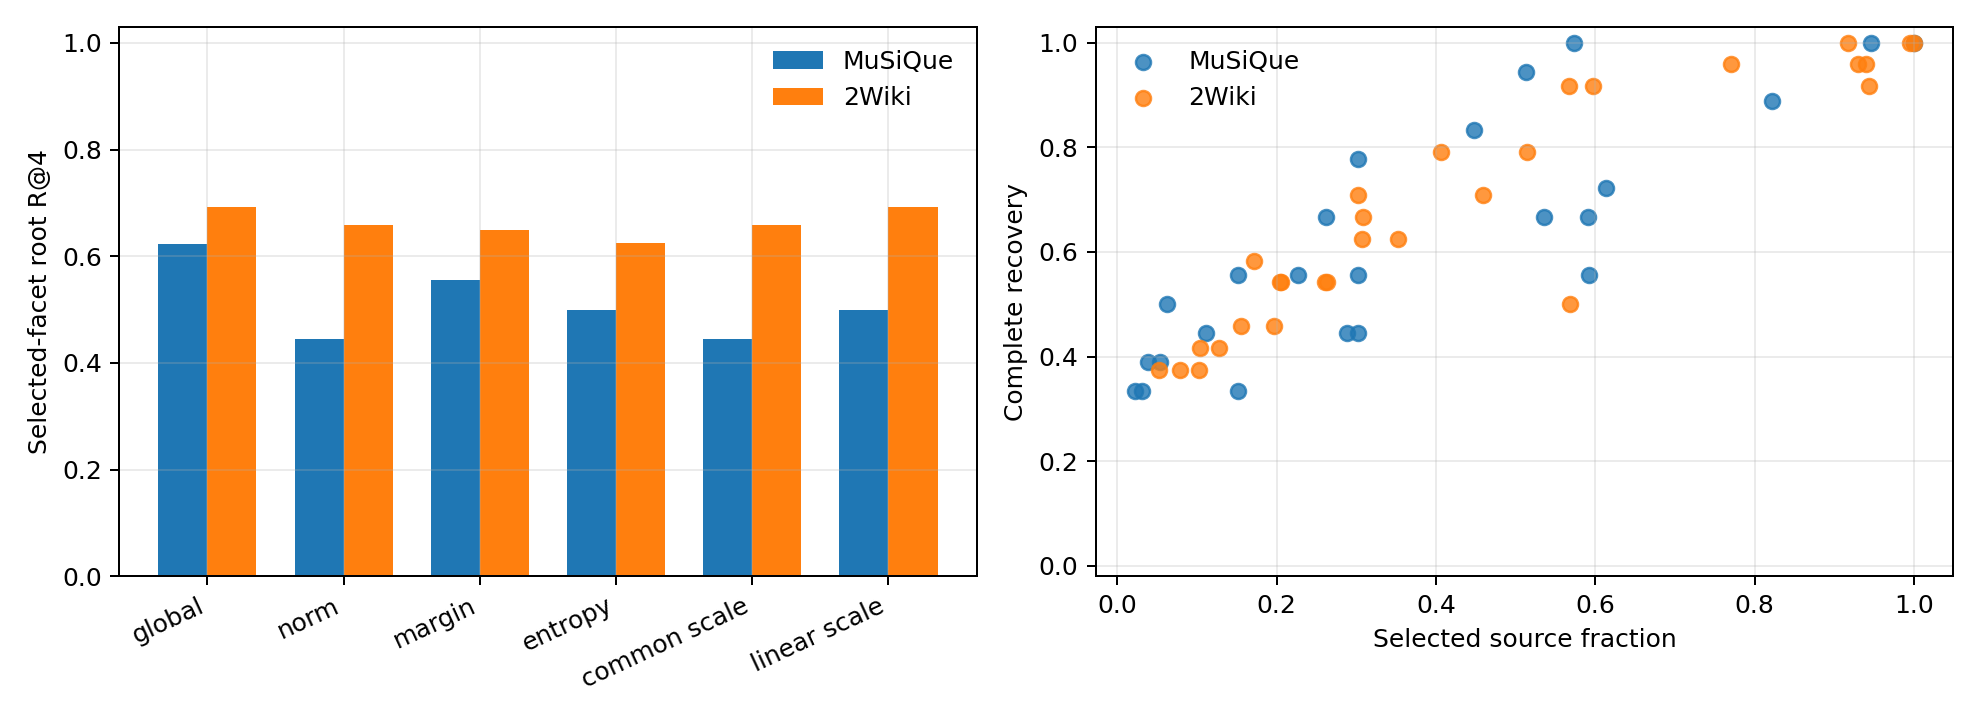
\includegraphics[width=0.90\linewidth]{../shared/results/paper2_5_iterative_pra/final_metrics/facet_predictability_frontier.png}
\caption{Executable root selectors remain below the oracle query-view ceiling; high complete
recovery also requires broad conceptual activation.}
\label{fig:main-entry-frontier}
\end{figure}

\subsection{Memory-to-memory topology and granularity}

Once 2Wiki search enters a correct 128-token node, direct successor R@4/R@6/R@8 is
.720/.880/1.000 and complete-path survival is .588/.824/1.000.  This establishes a strong local
associative neighborhood after entry.  It does not establish executable root routing or faithful
reasoning order.  On MuSiQue, evidence recovery often saturates by native search depth two even for
annotated depth-four questions, exposing shortcuts or contracted neighborhoods.

\begin{table}[H]
\centering
\caption{Held-out 2Wiki native-edge and path fidelity at 128-token nodes.}
\label{tab:main-2wiki}
\small
\begin{tabular}{rrrr}
\toprule
$K$ & Transition R@$K$ & Complete path & Broad evidence recovery \\
\midrule
4 & .720 & .588 & .917 \\
6 & .880 & .824 & .958 \\
8 & 1.000 & 1.000 & 1.000 \\
\bottomrule
\end{tabular}
\end{table}

Chunking changes the graph itself.  Fine nodes improve payload precision but remove useful edges;
coarse nodes contract evidence and distractors into the same conceptual unit.  At 16 tokens,
MuSiQue/2Wiki select only .063/.172 of source but recover complete evidence in .500/.583 cases.
Broad 128-token conditions reach complete recovery while selecting .573/.918 of source.  Deeper
search cannot recover an edge absent from the chosen graph scale.

\begin{figure}[H]
\centering
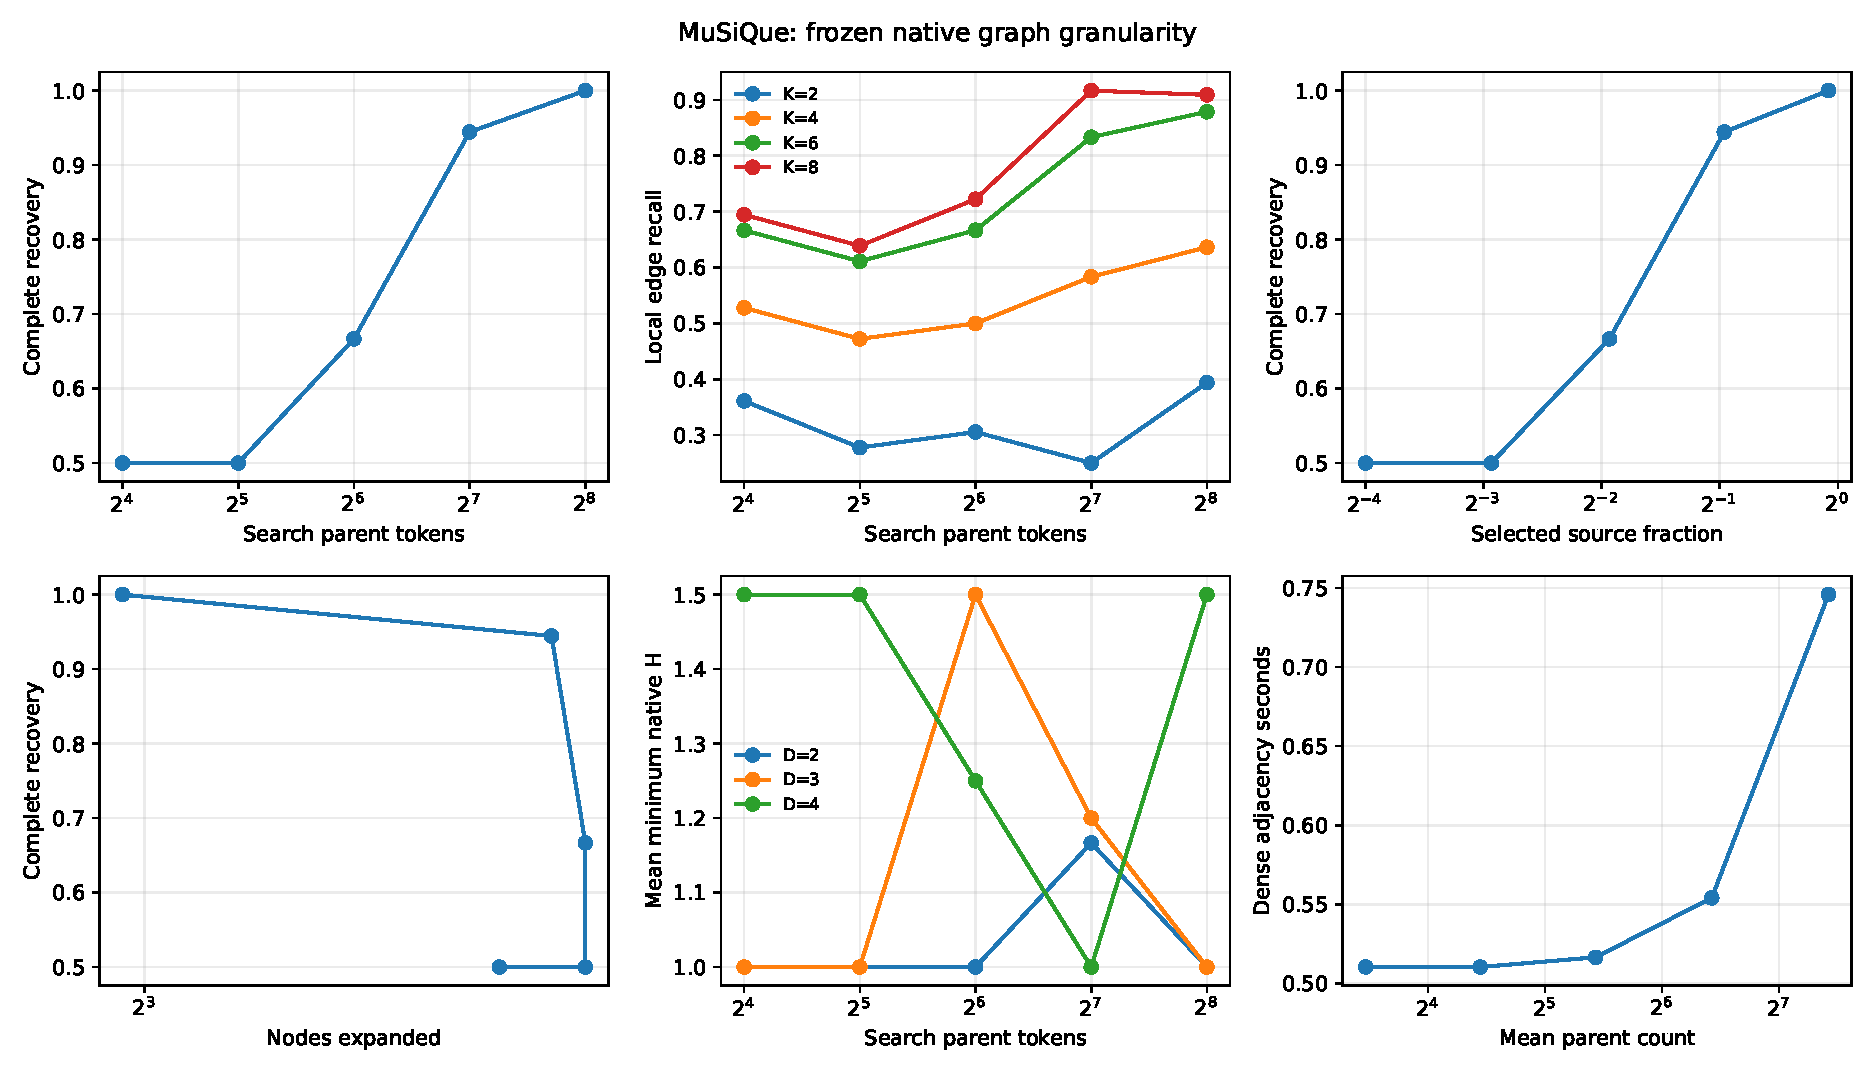
\includegraphics[width=0.49\linewidth]{../shared/results/paper2_5_iterative_pra/natural_graph_depth/musique_granularity.pdf}
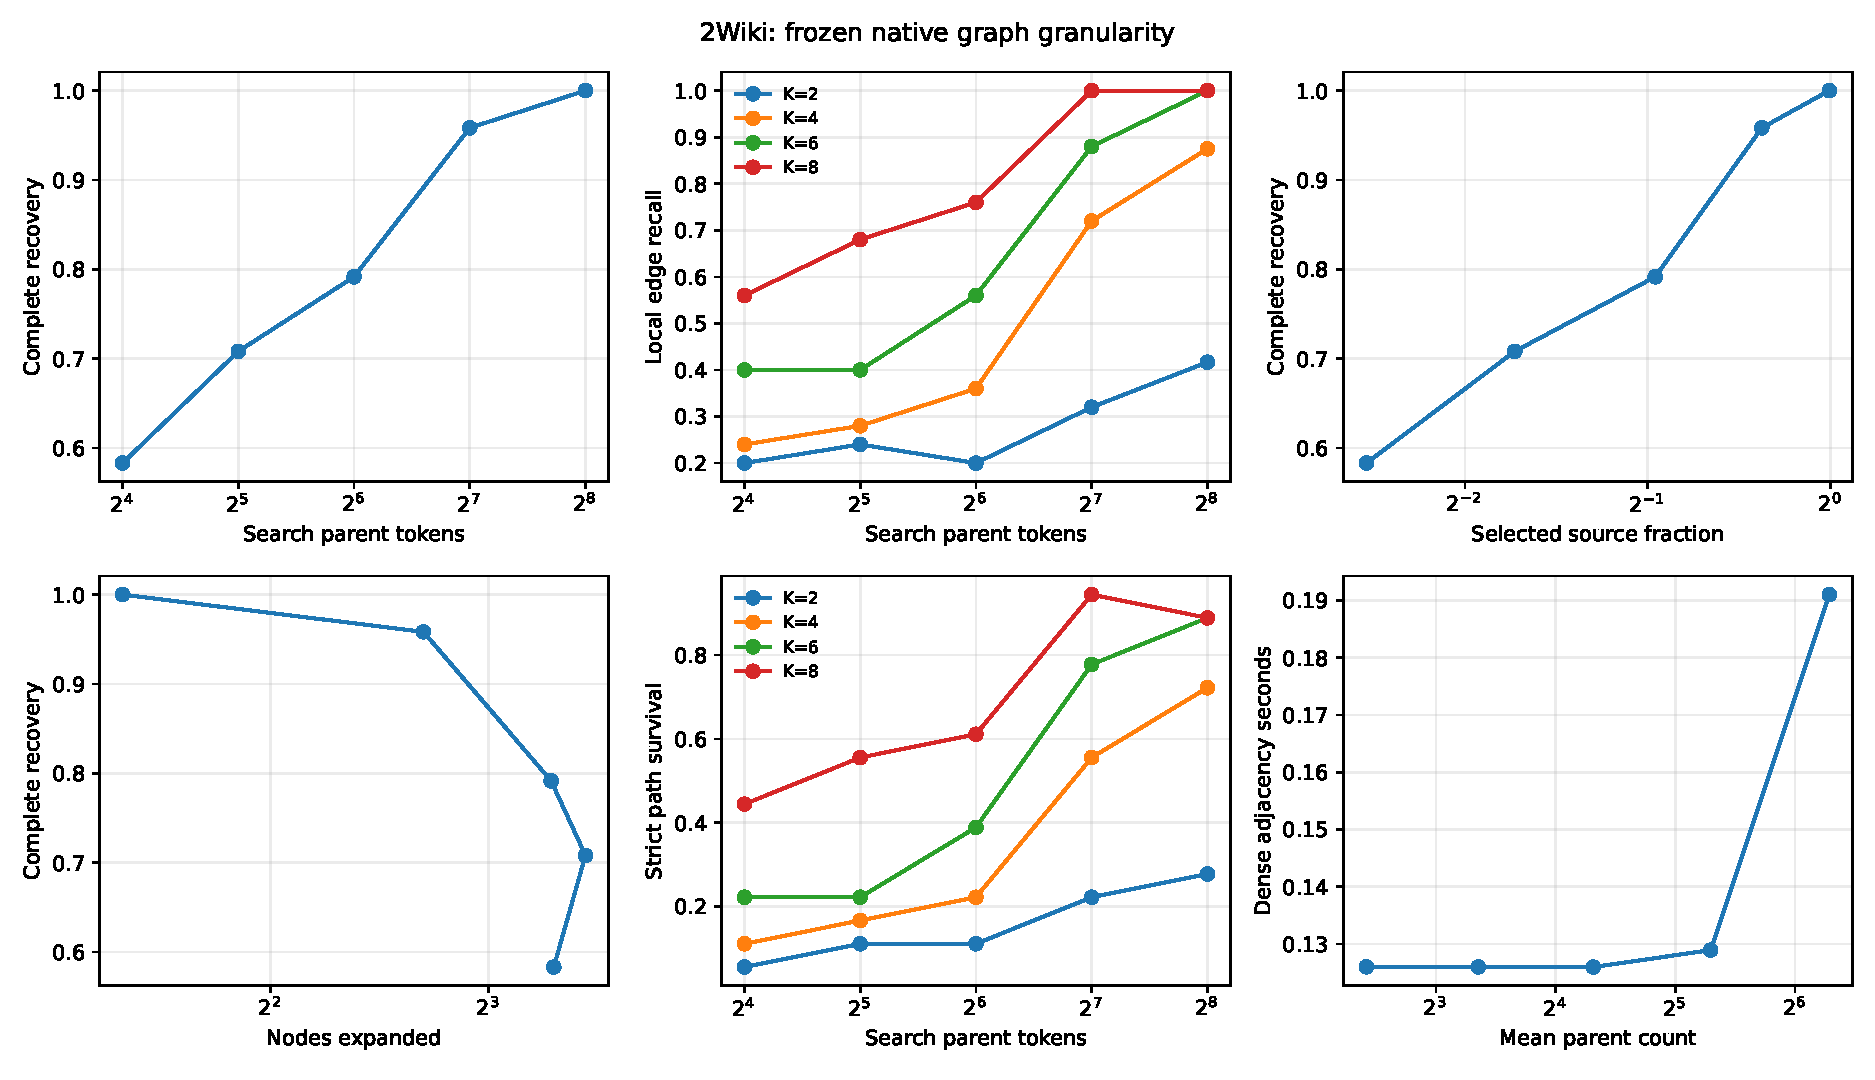
\includegraphics[width=0.49\linewidth]{../shared/results/paper2_5_iterative_pra/natural_graph_depth/2wiki_granularity.pdf}
\caption{Granularity changes both conceptual payload and complete evidence recovery.  Fine memory is
sparse but topologically fragile; coarse memory is reachable but distractor rich.}
\label{fig:main-granularity}
\end{figure}

\subsection{Layer topology}

Layer and granularity interact non-monotonically.  For 2Wiki at 32 tokens, layer-0 R@6 is .680 and
layer-27 R@6 is .400; at 128 tokens, layer 12 leads with .920.  Restricted-context dependence rises
strongly with layer but has weak, unstable relationships with edge R@6, MRR, contraction, and
shortcut rate.  The pretrained model therefore reproduces the controlled distinction between
contextualization and traversable topology.

\begin{figure}[H]
\centering
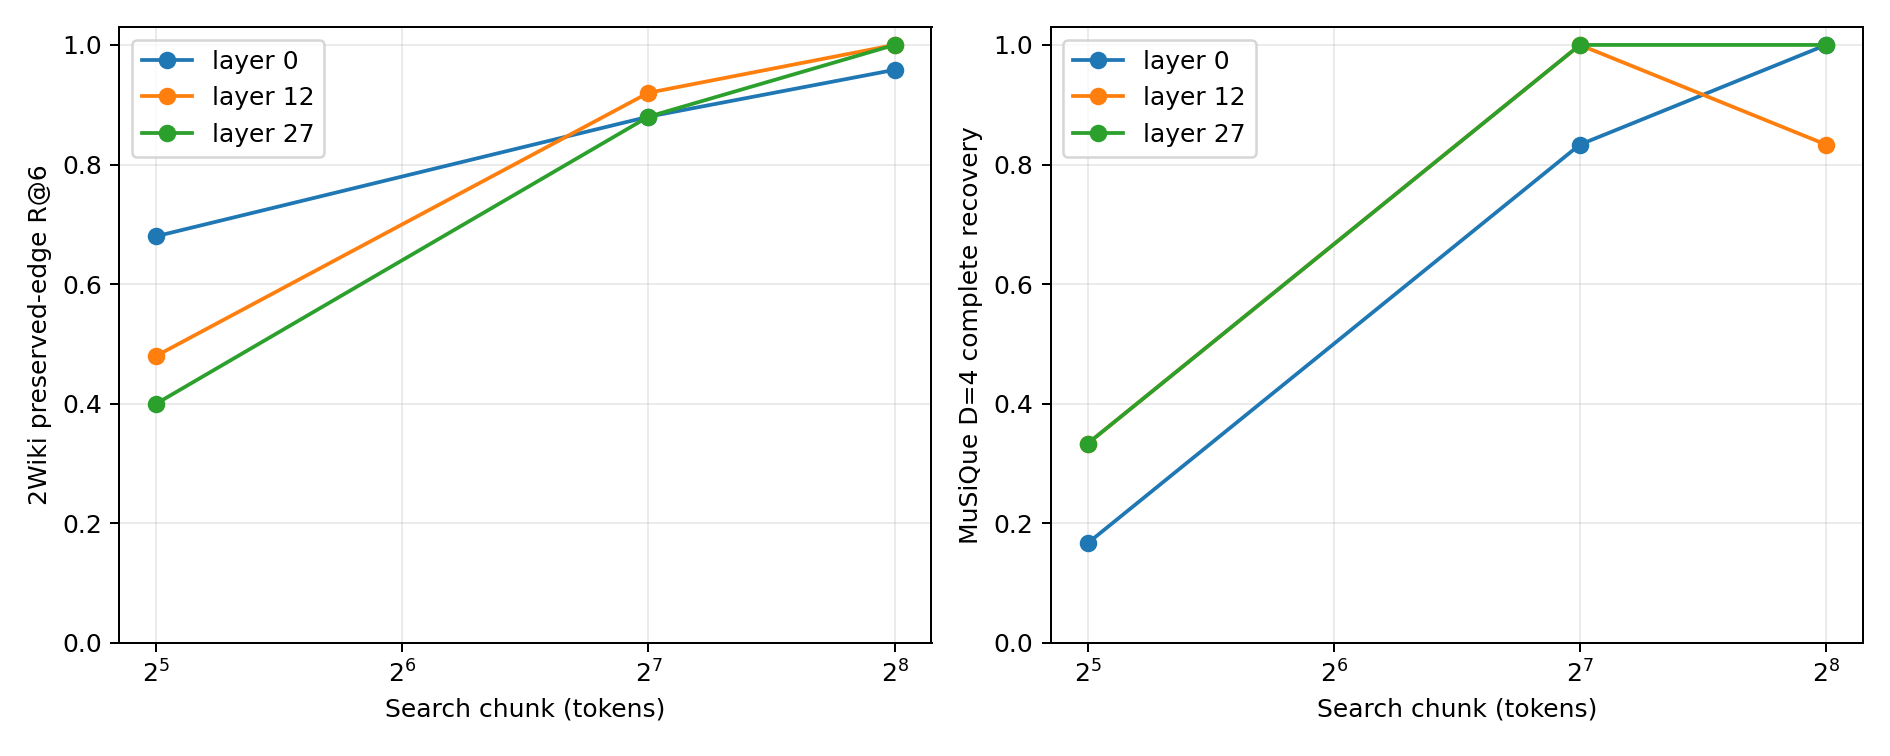
\includegraphics[width=0.49\linewidth]{../shared/results/paper2_5_iterative_pra/layerwise_graph/layer_granularity_cross.png}
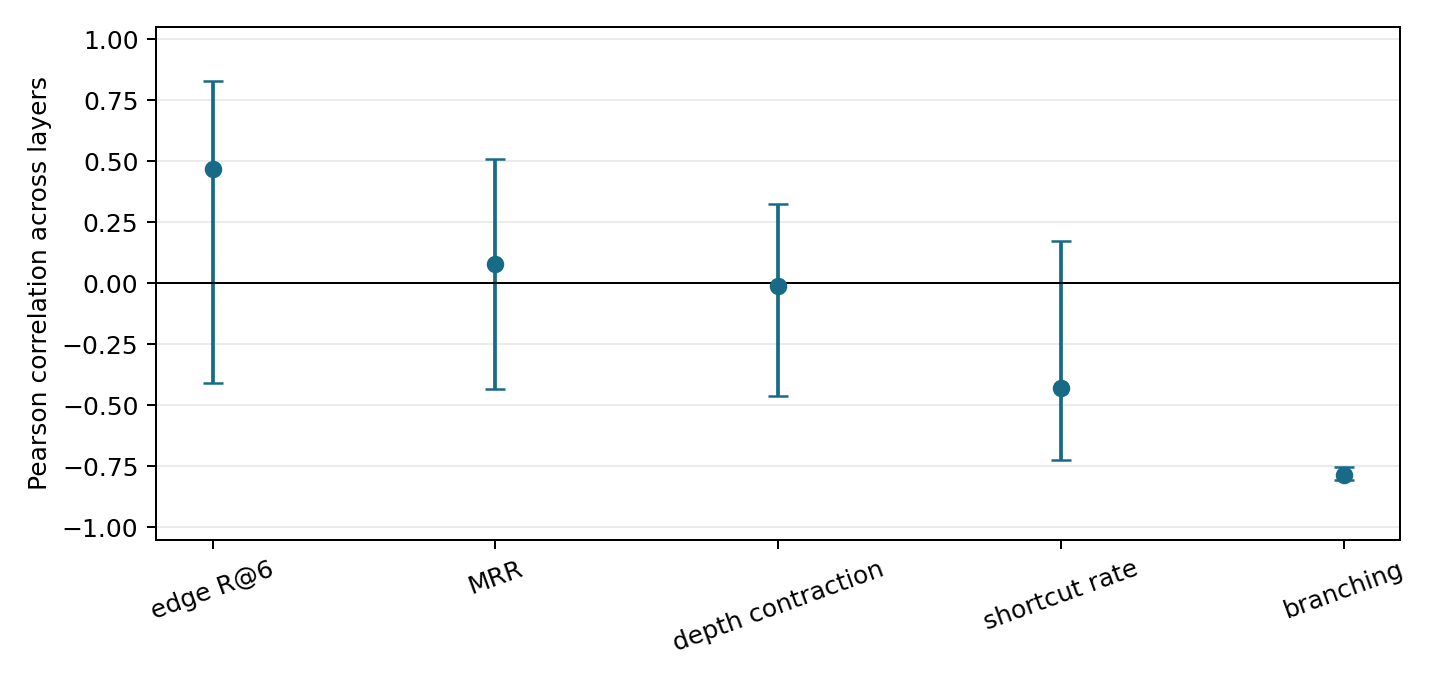
\includegraphics[width=0.49\linewidth]{../shared/results/paper2_5_iterative_pra/final_metrics/layer_context_matched_correlations.png}
\caption{Pretrained layer-by-granularity topology and matched contextualization correlations.  No
single late or highly contextual layer dominates every graph scale.}
\label{fig:main-layer}
\end{figure}

\subsection{Output validation}

Frozen generation reproduces the discovery/activation asymmetry.  On held-out 2Wiki, one-shot,
balanced, broad, and oracle F1 are .354, .313, .271, and .362.  Broad discovery recovers all evidence
but activates .934 of source; final-token attention assigns .044 to annotated evidence, .754 to
selected non-evidence, and .202 to the local prompt.  Oracle activation is denser in evidence
(.110/.461/.430) but still yields only a small, uncertain F1 gain.  All-layer consumption collapses
2Wiki output relative to the selected sparse band.  MuSiQue normalized accuracy is zero even under
direct full context, so this backbone cannot identify a useful output policy for that dataset.

\begin{table}[H]
\centering
\caption{Compact held-out 2Wiki output summary.  Selected source is conceptual activation; active
K/V is physical peak native state in thousands.}
\label{tab:main-output}
\small
\begin{tabular}{lrrrr}
\toprule
Condition & Evidence recall & Selected source & Active K/V & F1 \\
\midrule
Native, no source & .000 & .000 & 1.34 & .353 \\
One-shot PRA & .719 & .589 & 4.25 & .354 \\
Graph balanced & .760 & .586 & 4.27 & .313 \\
Graph broad & 1.000 & .934 & 6.22 & .271 \\
Oracle evidence & 1.000 & .320 & 2.88 & .362 \\
\bottomrule
\end{tabular}
\end{table}

A control-qualified GPT-5.6 Sol judge rates 2Wiki balanced versus one-shot at 90.0 semantic
equivalence and +2.9 relative quality, but favors the selected sparse band over all-layer output by
37.4 points.  Claude Sonnet 5 covers only 51.7\% of pairs and fails both calibration anchors; it is
retained as a failed-instrument diagnostic rather than efficacy evidence.  Pretrained experiments
thus do not establish dramatic QA gains.  They show that richer search improves access more
consistently than output, while layer placement and distractor competition materially affect use.

\section{Related Work}

Longformer, BigBird, and Routing Transformer sparsify token attention
\cite{beltagy2020longformer,zaheer2020bigbird,roy2021routing}; Transformer-XL, Compressive
Transformer, and feedback-memory models carry state across segments
\cite{dai2019transformerxl,rae2020compressive,hwang2024fam}.  These systems primarily modify access
within an extended sequence or recurrent state.  PRA instead probes an externally backed logical
memory whose compact identities and native K/V payloads remain separately addressable.

REALM, RAG, RETRO, and Atlas retrieve text or representations before or during generation
\cite{guu2020realm,lewis2020rag,borgeaud2022retro,izacard2023atlas}.  IRCoT and Self-RAG interleave
retrieval with generated reasoning or self-reflection \cite{trivedi2023ircot,asai2024selfrag}.
Iterative PRA does not generate an intermediate text query or rerun the transformer during compact
search.  This makes associative transitions cheap and auditable, but less expressive than an agent
that can reformulate the task.

H2O, SnapKV, and QUEST select or retain K/V entries for an available context
\cite{zhang2023h2o,li2024snapkv,tang2024quest}.  PRA separates root activation, associative identity
search, and later native-K/V disclosure.  The distinction motivates separate metrics for topology,
conceptual activation, physical K/V, attention allocation, residual change, and output.  At a
computational level, this resembles bounded associative memory: ongoing local processing is
occasionally influenced by a limited activated working set.  We use this analogy only to organize
resource and control questions, not to claim biological equivalence.

\section{Discussion}

The experiments support a progression from \emph{potential memory} to \emph{activated memory},
\emph{attended memory}, \emph{useful state change}, and \emph{preserved computation}.  Receptive
field changes potential associative topology.  Evolving-state PRA can traverse that topology.
Ordinary selection, however, exposes too many plausible distractors, so evidence does not dominate
the shared softmax.  Oracle forcing demonstrates that when evidence does dominate, the frozen
transformer can convert it into substantially better margins and predictions.

Controlled activation is therefore the primary unresolved mechanism.  It is not equivalent to
choosing the largest $K$, deepest search, or broadest source coverage.  Each plausible memory given
another opportunity to enter attention also competes with evidence.  The Qwen root-facet ceiling and
the controlled oracle intervention show that useful representations already exist; selecting a
small, evidence-dense working set remains difficult.

\subsection{Parameter directionality and adaptive effort}

One fixed PRA configuration is unlikely to be optimal because each control moves opportunity,
distractor pressure, physical state, and compute differently (Table~\ref{tab:parameter-direction}).
More facets $F$ preserve more query intents but create more candidate competition; this helped
Hotpot root inclusion while leaving QASPER unchanged at the same 20\% budget.  More roots $R$ improve
entry coverage but broaden the selected working set.  More neighbors $K$ improve successor
availability at superlinear comparison cost: the held-out Hotpot oracle-root control recovers all
oracle parents at $K=4,B=6$, whereas faithful 2Wiki transition and path recovery require $K=8$.
Neither operating point is universal.  Greater hop depth $H$ can recover long paths, but global
contextualization can contract them into shallow shortcuts before routing begins.  A larger final
budget $B$ tolerates ranking error while increasing active K/V and softmax competition.  Raising an
acceptance threshold $\theta$ reverses that tradeoff, improving precision while risking weak bridge
evidence; earlier threshold-calibration gates did not identify a reliable closure rule.

Consumer placement is a separate axis.  More PRA layers offer repeated assimilation but consume
more layer-token K/V and can perturb or erase useful residual changes.  The best search layer need
not be the best consumer layer or preservation schedule.  Finally, chunk granularity $G$ changes the
graph itself: coarse nodes improve containment at low node count but disclose irrelevant payload,
whereas fine nodes improve payload precision while increasing graph size and sensitivity to missing
edges, $K$, and $H$.

\begin{table}[H]
\centering
\caption{Dominant parameter directions, not universal monotonic laws.  Effects depend on dataset,
layer, granularity, and routing quality.}
\label{tab:parameter-direction}
\scriptsize
\begin{tabular}{lccccc p{0.22\linewidth}}
\toprule
Parameter $\uparrow$ & Root & Path & Distractors & Active K/V & Search & Typical benefit \\
\midrule
$F$ facets & $\uparrow$ & indirect $\uparrow$ & $\uparrow$ & indirect $\uparrow$ & $\uparrow$ & Ambiguous, multi-intent queries \\
$R$ roots & $\uparrow$ & $\uparrow$ & $\uparrow\uparrow$ & $\uparrow$ & $\uparrow$ & Uncertain root rank \\
$K$ neighbors & --- & $\uparrow$ & $\uparrow$ & $\uparrow$ & $\uparrow\uparrow$ & Noisy successor rank \\
$H$ hops & --- & deep paths $\uparrow$ & $\uparrow\uparrow$ & $\uparrow$ & $\uparrow\uparrow$ & Distributed evidence \\
$B$ budget & $\uparrow$/--- & $\uparrow$ & $\uparrow\uparrow$ & $\uparrow\uparrow$ & ---/$\uparrow$ & Incomplete coverage \\
$\theta$ threshold & precision $\uparrow$, recall $\downarrow$ & varies & $\downarrow$ & $\downarrow$ & $\downarrow$ & Confidence filtering \\
PRA layers & --- & potential $\uparrow$ & interference & $\uparrow\uparrow$ & $\uparrow$ & Repeated assimilation \\
Finer $G$ & varies & edges can $\downarrow$ & payload $\downarrow$ & $\downarrow$/node & nodes $\uparrow$ & Precise disclosure \\
\bottomrule
\end{tabular}
\end{table}

These coupled directions motivate adaptive rather than globally maximal effort:
$\mathrm{query/state}\rightarrow(F,R,K,H,B,\theta,L,G)$.  A QASPER-like direct query may use a
narrow policy; a Hotpot bridge query may warrant additional facets or roots; distributed MuSiQue
evidence may warrant more search and coverage budget only when confidence justifies the added
distractor load.  Paper 3.5 asks whether a controller can make that decision; this paper does not
train or evaluate one.

Search, consumption, and preservation operate on different computational timescales.  A layer can
have useful native Q/K topology while being a poor location for injecting value vectors.  An early
consumer can create a useful change that later layers erase.  These observations favor architectures
that treat local ongoing computation, sparse nonlocal activation, and assimilation time as separate
controls.  They do not establish that one layer schedule generalizes across model families.

The bounded-processing analogy is deliberately restrained.  A limited working set can be useful
because not every associatively plausible memory should dominate current processing.  Iterative
retrieval permits one activated memory to redirect the next search, while finite budgets force a
choice about what becomes influential.  Adaptive control is a natural next question, but it is not
evaluated here.

\section{Limitations}

The controlled models are 740K-parameter scientific instruments with a synthetic vocabulary, not
language-model scaling evidence.  Five seeds leave wide Student-$t$ intervals; the minimum exact
two-sided result with five same-direction nonzero effects is $p=.0625$.  The primary PRA corpus has
32 examples per seed and the mechanistic cohort has 16.  Model--example bootstrap analyses do not
turn repeated examples across seeds into independent model replicates.  Oracle forcing is a causal
ceiling, not an executable router.

The local mask uses a dense kernel, so controlled elapsed time does not estimate optimized LocalSA.
Exact SA-to-PRA conversion is intentionally frozen.  The experiment tests inherited topology and
memory use, not PRA-aware training.  Content shuffling also shows that some ordinary selected-memory
gain is not evidence specific.

Natural cohorts are diagnostic: 18 held-out MuSiQue identities, 24 2Wiki identities, smaller inherited
HotpotQA/QASPER sets, and one principal Qwen3-0.6B family.  Oracle-root analyses isolate successor
geometry rather than end-to-end routing.  Annotation graphs need not be the model's preferred
reasoning paths.  MuSiQue generation is backbone limited even with full context.  Python graph search
and trace-oriented materialization are not production-serving kernels.  One external judge passes
calibration; the second is partial and fails it.

The causal $W=16$ versus global topology result is established in the controlled 25-model family.
Pretrained Qwen layer/chunk diagnostics are directionally consistent with architecture-dependent
topology but do not constitute a causal pretrained LocalSA-versus-GlobalSA comparison.

\section{Scope Boundaries and Follow-up Work}

\paragraph{Paper 3: physical disclosure.}
Given selected conceptual memory, how much native K/V detail should become active?  Evidence-centered
materialization, overlap deduplication, and quality at a smaller physical payload belong there.  Paper
2.5 measures selected identities and uses matched causal payloads; it does not optimize disclosure.

\paragraph{Paper 3.5: adaptive control.}
How should query difficulty or confidence adapt facets, roots, $K$, hops, budgets, retries, and runtime
effort?  The distractor-dominated result directly motivates a controller that spends additional search
only when it improves evidence concentration.  No such controller is trained or evaluated here.

\paragraph{Paper 4: learned robustness.}
Can frozen-to-LoRA-to-full-weight-to-native PRA training make memory representation, consumption, and
assimilation robust to imperfect sparse memory?  The motivation is not that frozen consumers cannot
use memory: oracle evidence proves they can.  Training may instead improve robustness, portability,
and preservation under noisy executable activation.  Because oracle evidence substantially improves
frozen-model output, PRA-aware training should evaluate robustness as memory quality degrades from
oracle to partially correct to ordinary noisy retrieval, not merely oracle performance.

\section{Conclusion}

Transformer memory exposes an associative topology whose explicit traversability depends on native
receptive field.  In the controlled family, final-layer edge R@4 is .428 at $W=16$ and .187 under
global attention.  Evolving-state PRA can exploit that structure to recover more paths under the
same physical K/V budget.

Better traversal is useful when it changes evidence.  It does so in 59/400 (14.8\%) model--example
units, which gain 2.164 correct-label margin, even though the current policy produces too few such
cases for a stable aggregate accuracy gain.  The causal intervention explains the operational gap:
ordinary memory is
distractor dominated, while matched oracle evidence raises frozen accuracy from .140 to .398 and
margin from $-3.103$ to $-.703$.  The frozen transformer can consume correct PRA memory.

Paper 2.5 therefore ends at controlled activation and preservation.  The immediate challenge is not
another graph-search variant or a claim of absolute consumer incapacity.  It is to activate a sparse
working set whose influence is concentrated on useful evidence, place that activation where the
residual computation can use it, and preserve the resulting change.  Physical K/V disclosure,
adaptive effort, and learned robustness remain deliberately separate research programs.
